\subsection{0-reducibility of ring $R_4$}

\begin{frame}
    \frametitle{0-reducibility of ring $R_4$}

    \begin{theorem}<1->
        The ring $R_4$ is 0-reducible
    \end{theorem}
    \uncover<2->{
        \textit{Proof.} We will show that there is a common ring coloring for any $M+R_4$ and $\confg$. Let the ring colorings of the two graphs be given by
        \begin{equation}
            \I = \Phi(M+R_4) \quad \text{and} \quad \II = \Phi(\confg).
        \end{equation}
    }
    \uncover<3->{
        The situation is sketched below.
        \begin{figure}[!ht]
        \centering
        \begin{tikzpicture}[mid arrow/.style={
            postaction={ decorate, decoration={ markings, mark=at position 0.6 with { \arrow[black]{>>} } } } }]
            \draw[fill=white] (-0.5, 0) ellipse (2cm and 1.5cm);
            \node (m) at (-1.7, 0) {$M$};
            \node at (-0.75, 0.75) {$R_4$};
    
            \node[circle, fill, scale=0.015cm] (l1) at (0, 0.9) { };
            \node[circle, fill, scale=0.015cm] (l2) at (0.9, 0) { };
            \node[circle, fill, scale=0.015cm] (l3) at (0, -0.9) {};
            \node[circle, fill, scale=0.015cm] (l4) at (-0.9, 0) {};
    
            \draw[mid arrow] (l1) -- (l2);
            \draw (l2) -- (l3) -- (l4) -- (l1);
        \end{tikzpicture}
        \begin{tikzpicture}[mid arrow/.style={
            postaction={ decorate, decoration={ markings, mark=at position 0.6 with { \arrow[black]{>>} } } } }]
            \draw[opacity=0] (-0.5, 0) ellipse (2cm and 1.5cm);
            \node at (-0.75, 0.75) {$R_4$};
            \node[inner sep=1mm] (c) at (0, 0) {$\core$};
    
            \node[circle, fill, scale=0.015cm] (l1) at (0, 0.9) { };
            \node[circle, fill, scale=0.015cm] (l2) at (0.9, 0) { };
            \node[circle, fill, scale=0.015cm] (l3) at (0, -0.9) {};
            \node[circle, fill, scale=0.015cm] (l4) at (-0.9, 0) {};
    
            \draw[mid arrow] (l1) -- (l2);
            \draw (l2) -- (l3) -- (l4) -- (l1);
            \draw[opacity=0.2] (l1) -- (c);
            \draw[opacity=0.2] (l2) -- (c); 
            \draw[opacity=0.2] (l3) -- (c);
            \draw[opacity=0.2] (l4) -- (c);
        \end{tikzpicture}
    \end{figure}}
\end{frame}

\begin{frame}
    \frametitle{0-reducibility of ring $R_4$}

    \uncover<1->{Both parts have a plain ring $R_4$, which we have shown to be reducible. Therefore, we may contract any two opposing vertices.}
    
    \uncover<2->{This gives us a guarantee on two colorings in both sets I and II.

    \begin{equation}
        \left\{\begin{matrix}
            abab \;\;\text{or}\;\; abac, \\
            baba \;\;\text{or}\;\; baca
        \end{matrix}\right\} \subset I,II.
    \end{equation}}

    \uncover<3->{
        Therefore, we have 4 possible options for guaranteed colorings in I and II, 3 of which are unique.

        \begin{equation}
            \circled{1} = \{ abab \}, \quad \circled{2} = \left\{ \begin{matrix}abab \\ baca\end{matrix} \right\}, \quad \circled{3} = \left\{ \begin{matrix}abac \\ baba \end{matrix} \right\}, \quad \circled{4} = \left\{ \begin{matrix}abac \\ baca \end{matrix} \right\}.
        \end{equation}
    }
\end{frame}

\begin{frame}
    \frametitle{0-reducibility of ring $R_4$}
    \begin{equation*}
        \circled{1} = \{ abab \}, \quad \circled{2} = \left\{ \begin{matrix}abab \\ baca\end{matrix} \right\}, \quad \circled{3} = \left\{ \begin{matrix}abac \\ baba \end{matrix} \right\}, \quad \circled{4} = \left\{ \begin{matrix}abac \\ baca \end{matrix} \right\}.
    \end{equation*}

    \uncover<1->{We consider all pairs that can occur for $\I$ and $\II$. All but one pair already have a common ring coloring.}
    
    \uncover<2->{The only pair that does not directly have a common coloring is $\circled{1}$ and $\circled{4}$. }
\end{frame}

\begin{frame}
    \frametitle{0-reducibility of ring $R_4$}
    
    \uncover<1->{Let $\{ abab \} \subset \I$ and $\{ abac, baca \} \subset \II$ be guaranteed colorings. }
    
    \uncover<2->{Suppose that in the coloring $\I(abab)$ we have $\chain{v_1}{v_3}{ad}$.

    \begin{equation}
        \begin{aligned}
            \I(abab) &= \scheme{a,b,a,b}{13d} \compat \II(abac) \\
            \I(abab) &= \scheme{a,b,a,b}{13d-} \compat \I(abcb) = \II(baca).
        \end{aligned}
    \end{equation}    
    
    Therefore, the guaranteed colorings always lead to a common coloring $\qedsymbol$.
    }
    
\end{frame}

\begin{frame}
    \frametitle{Examples of reducible configurations on $R_4$}
    \centering
    \begin{figure}
        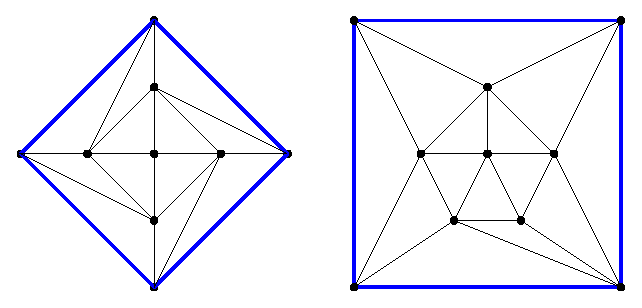
\includegraphics[width=0.7\textwidth]{images/example4.eps}
    \end{figure}

    Because $R_4$ is 0-reducible, the interior of \textbf{any} configuration on $R_4$ can be removed.
\end{frame}